\documentclass{article}
\renewcommand{\familydefault}{\sfdefault}
\usepackage{graphicx} % Required for inserting images
\usepackage{helvet}
\usepackage{geometry}
\usepackage{hyperref}
\usepackage{listings}
\geometry{top=2.5cm, bottom=2cm}
\usepackage{multirow}





\begin{figure}[h]
        \centering
        
\includegraphics[width=10cm]{images/Logo.png}
\end{figure}



\title{Quanto-Solutions}

\date{November 2023}



\renewcommand{\listfigurename}{Abbildungsverzeichnis}

\begin{document}

\maketitle


\begin{table}[h]
    \centering
   
    \begin{tabular}{|p{3cm}|c|p{3cm}|}
        \hline
        \textbf{Name} & \textbf{Matrikelnummer} & \textbf{Githubaccount} \\
        \hline
        Chris Schröder    & 767384    & Chris0297  \\
        Michele Pomarico  & 766583    & Michele-92 \\
        Fabian Sonek      & 767903    & e2Neo      \\
        Baran Kal         & 769042    & Roplck     \\
        Daniel Ryssel     & 768960    & danGitRys  \\
        \hline
    \end{tabular}
\end{table}


\newpage

\tableofcontents  %Inhaltsverzeichnis
 
\newpage
\listoffigures  % Abbildungsverzeichnis
\newpage


\section{Introduction}

\section{Kurzfassung}
    Dieses Dokument behandelt die Dokumentation der Projektmanagement Software, welche im Rahmen des Moduls “Projekt Softwaretechnik und Medieninformatik” im Studiengang Softwaretechnik und Medieninformatik an der Hochschule Esslingen für die Firma Quanto-Solutions entwickelt wird.

\newpage



\section{Zielgruppe/Problemstellung}
Zum aktuellen Zeitpunkt werden von der Firma Quanto-Solutions für die Projektverwaltung Excel-Tabellen verwendet, um die Mitarbeiter einem Projekt zuzuordnen und die Arbeitszeit zu erfassen. Dabei gibt es das Problem des Verwaltens der Zugriffsrechte auf die Excel Dateien, da aus Datenschutzgründen nicht jeder Mitarbeiter alle Informationen einsehen darf, was darin resultiert, dass nur die Managementebene in der Firma diese nutzen darf.  Dadurch gestaltet sich das Eintragen der Arbeitsstunden als sehr Zeit aufwändig.
Um diese Probleme zu lösen, wurden wir beauftragt, eine Projektmanagement-Software zu entwickeln, die für unsere Zielgruppe, alle Mitarbeiter von Quanto-Solutions, zugänglich ist und eine Möglichkeit bietet, IST-Aufwände schnell und komfortabel buchen zu können.

    \subsection{ User Stories}
        \subsubsection{Nutzer (Mitarbeiter, Projekt Manager, Manager) }
         \begin{itemize}
        \item Als Nutzer möchte ich mich einloggen können, um Zugriff auf das Projektmanagement-Tool zu erhalten. (Login)
        \item Als Nutzer möchte ich meine Arbeitszeiten erfassen können, um diese auf ein Projekt zu buchen. (Time Registration)
        \item Als Nutzer möchte ich meine eingeplanten Arbeitszeiten sehen können, um einen Überblick über meine erfassten und geplanten Arbeitszeiten zu bekommen. (Working Times)
        \item Als Nutzer möchte ich meine Arbeitszeiten korrigieren können, um eine korrekte Erstellung der Rechnung zu gewährleisten. (Time Correction)
        \item Als Nutzer möchte ich mit Hilfe der Sidebar schnell die Ansichten wechseln können, um effektiver zu arbeiten. (Sidebar)
        \item Als Nutzer möchte ich in meinem Home Screen alle meine Projekte aufgelistet bekommen, um eine Übersicht des aktuellen Standes der Projekte zu erlangen. (Home)
        \end{itemize}

        \subsubsection{ Projekt Manager}
        \begin{itemize}
        \item Als Projekt Manager möchte ich Projekte verwalten können, um die Mitarbeiter auf Tagesebene einem Projekt in einer bestimmten Position zuzuordnen. (Manage Project)
        \item Als Projekt Manager möchte ich die Arbeitszeiten der Mitarbeiter sehen können und Sie manuell nachtragen, um die richtige Abrechnung der Positionen gewährleisten zu können. (Working Times+)
        \end{itemize}

        \subsubsection{ Manager}
        \begin{itemize}
        \item Als Manger möchte ich ein neues Projekt anlegen können mit folgenden Informationen: Kunde, Projektname, Zeitraum, Projektmanager, hinzufügen von Mitarbeitern, Positionen und Tagessätzen, um einen bessere Projektübersicht und damit eine strukturierte Planungsmöglichkeit zu erhalten. (New Project)
        \item Als Manager möchte ich Projekte verwalten können, um die Mitarbeiter auf Tagesebene einem Projekt in einer bestimmten Position zuzuordnen. (Manage Project)
        \item Als Manager möchte ich die Arbeitszeiten der Mitarbeiter sehen können und Sie manuell nachtragen, um die richtige Abrechnung der Positionen gewährleisten zu können. (Working Times+)
        \end{itemize}

    \subsection{ Functional Requirements}

        \subsubsection{Projektanlage für Manager}
        Das System muss es Managern ermöglichen, neue Projekte anzulegen, wobei sie wichtige Informationen wie Kundenname, Projektbezeichnung und den Zeitraum festlegen können. Dies erleichtert die klare Definition und Überwachung der Projekte von ihrem Beginn an.
        \subsubsection{Projektmanagemnt-Befugnisse für Manager}
        Manager sollten in der Lage sein, für jedes Projekt einen verantwortlichen Projektmanager (PM) zu bestimmen und Mitarbeiter für das Projekt zuzuordnen sowie den Mitarbeitern Positionen zuordnen zu können. Diese Funktion gewährleistet, dass die Zuständigkeiten klar verteilt sind und die Teams gut organisiert sind.
        \subsubsection{Tägliche Einsatzplanung für Projektmanager}
        Projektmanager müssen auf Tagesebene eine detaillierte Einsatzplanung für die Mitarbeiter erstellen können. Dies ermöglicht eine präzise und effektive Zeiterfassung, um sicherzustellen, dass Projekte termingerecht abgeschlossen werden.
        \subsubsection{Zeitaufzeichung und Reminder für Mitarbeiter}
        Die Mitarbeiter sollten in der Lage sein, ihre “IST-Aufwände” zu erfassen, um den Arbeitsfortschritt und die Aufgabenverwaltung zu gewährleisten. Darüber hinaus sollte das System automatische Erinnerungen bereitstellen, um sicherzustellen, dass die Zeitaufzeichnung zeitnah und korrekt erfolgt.
        \subsubsection{Berechtigungsabhängige Funktionalitäten}
        Die Funktionalitäten des Systems sollten abhängig von der Benutzerrolle variieren. Das bedeutet, dass Manager, Projektmanager und Mitarbeiter jeweils nur auf die Funktionen und Informationen zugreifen können, die für ihre jeweiligen Aufgaben relevant sind. Dies gewährleistet die Sicherheit von Daten und erhöht die Effizienz, da Benutzer nicht mit irrelevanten Informationen überlastet werden.
    \subsection{ Nonfunctional Requirements}
    Als Non-Functional Requirements in diesem Projekt ist wichtig, dass die Anwendung als Web-Anwendung läuft.

\newpage

\section{High Level Arichtektur Programm}
    \subsection{ Struktursicht}
        \begin{figure}[h]
            \centering
            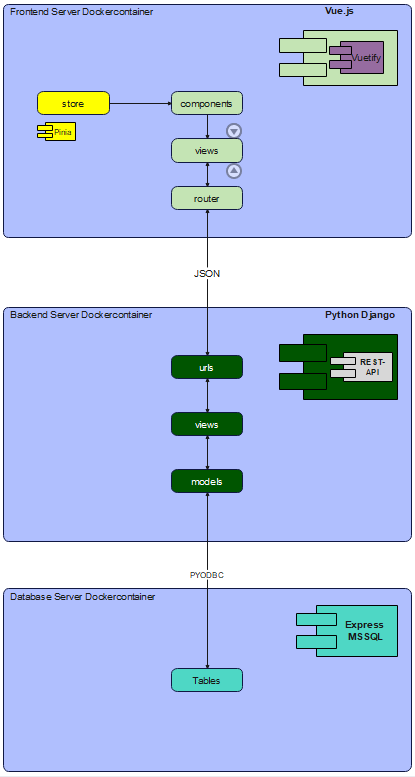
\includegraphics[scale=0.85]{images/Struktursicht.png}
            \caption{Komponentendiagramm}
            \label{fig:beispiel}
        \end{figure}
    \newpage
    \subsection{ Verhaltenssicht}
        \begin{figure}[h]
            \centering
            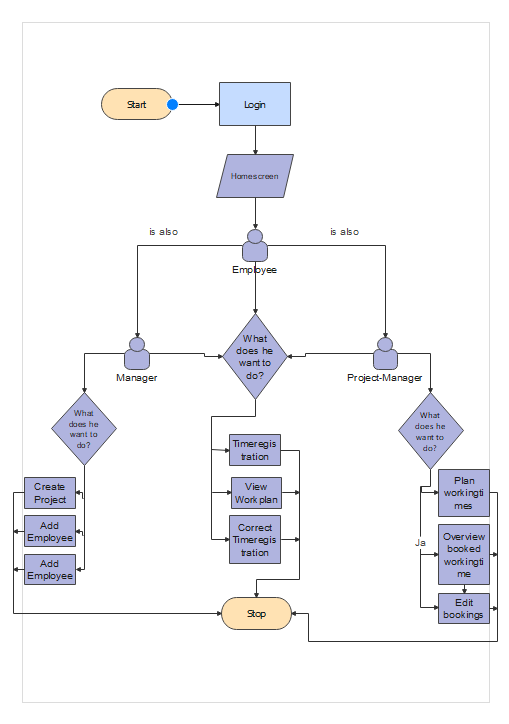
\includegraphics[scale=0.9]{images/Verhaltenssicht.png}
            \caption{Ablaufdiagramm}
            \label{fig:beispiel}
        \end{figure}
    \newpage
    \subsection{ Verteilungssicht}
        \begin{figure}[h]
  
            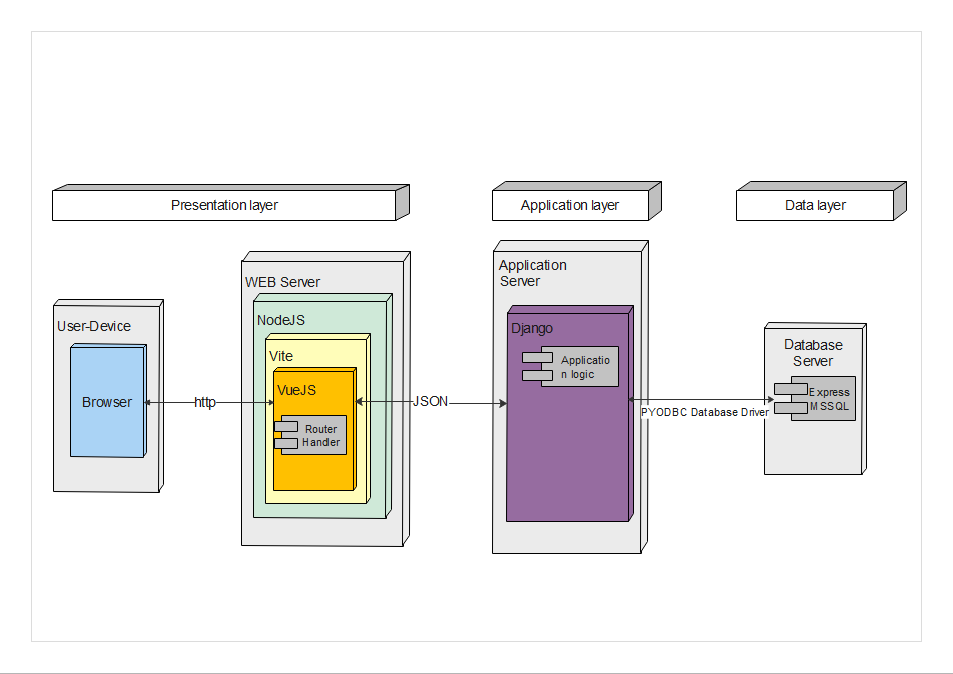
\includegraphics[width= \textwidth]{images/Verteilungssicht.png}
            \caption{Verteilungsdiagramm}
            \label{fig:beispiel}
        \end{figure}

\newpage

\section{Architektur/ Technologie}

    \subsection{Github}
    Zur Versionsverwaltung des Codes des Projektes wird Github verwendet. Darüber hinaus bietet GitHub Werkzeuge zur Fehlerverfolgung an, die es uns ermöglichen, Probleme und Verbesserungen in unserem Projekt zu dokumentieren und nachzuverfolgen. Die Verwendung von GitHub erleichtert die Zusammenarbeit und ermöglicht eine transparente und gut organisierte Entwicklungsumgebung für das Projekt.
    
    \begin{figure}[h]
        \centering
        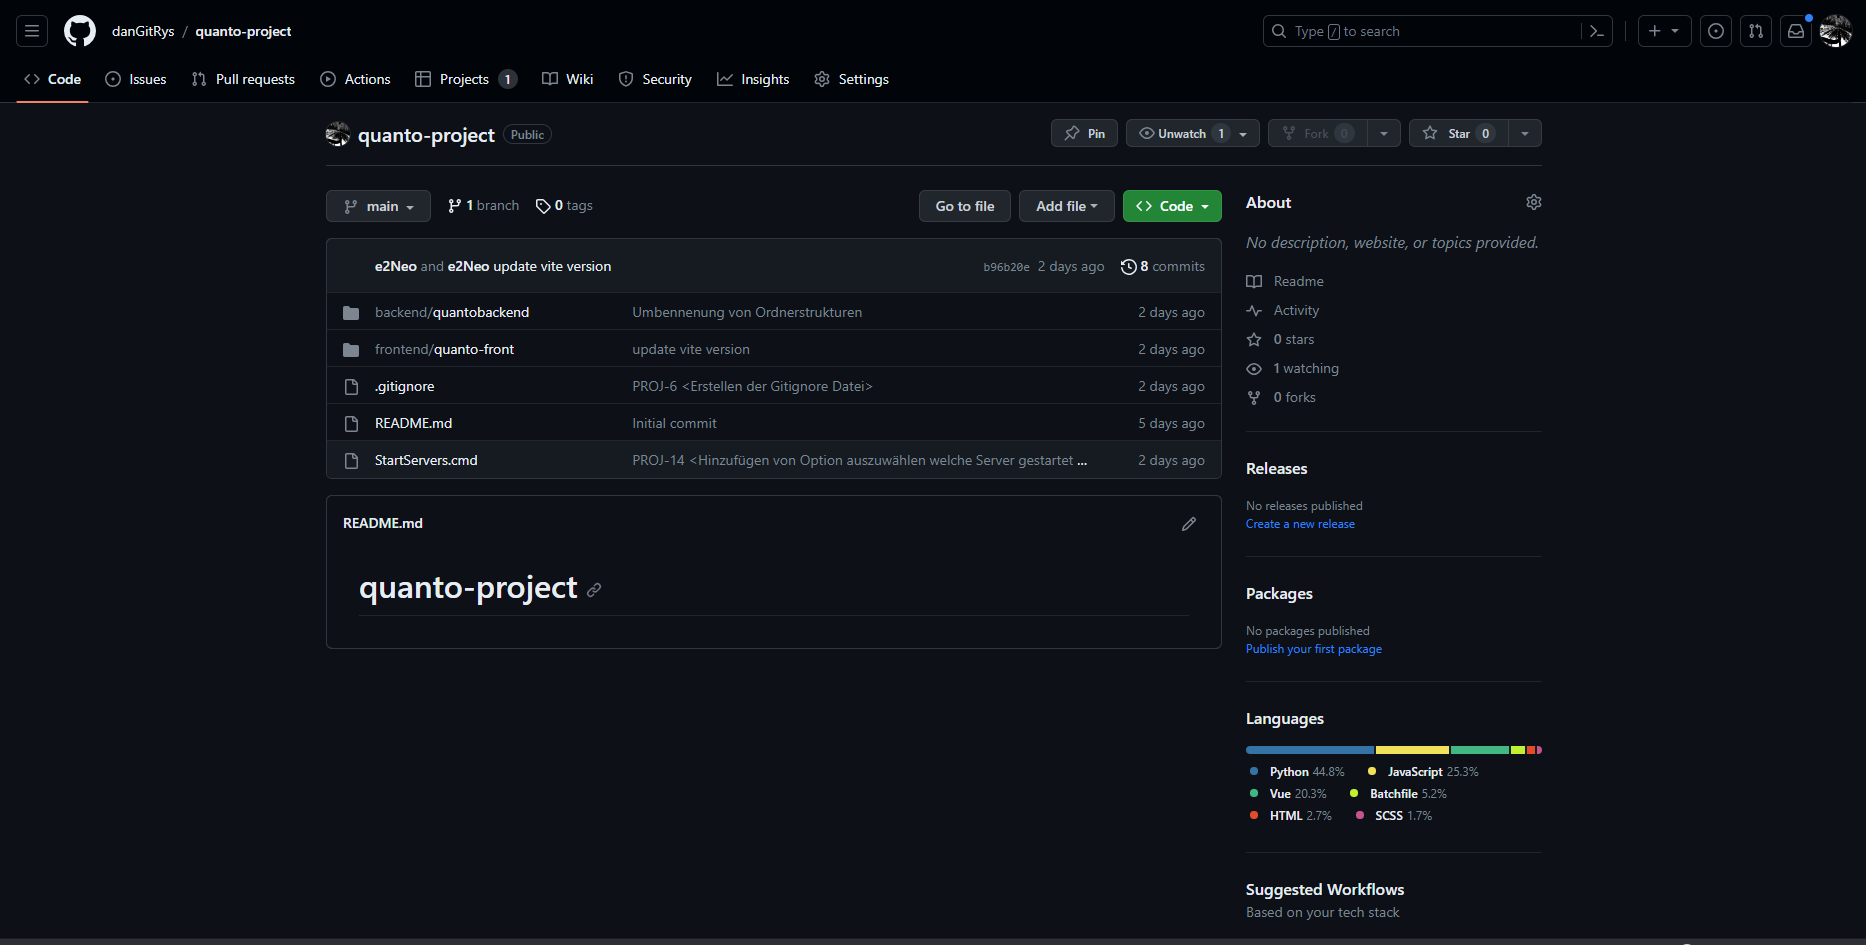
\includegraphics[width= \textwidth]{images/GitHub.png}
        \caption{Screenshot Github}
        \label{fig:beispiel}
    \end{figure}
    \subsection{Genutzte IDEs}
    Als IDE wird VS-Code von Microsoft verwendet. Aufgrund der Konfigurierbarkeit von VS-Code wird es für die Entwicklung des Front- und Backend verwendet.
    
    \begin{figure}[h]
        \centering
        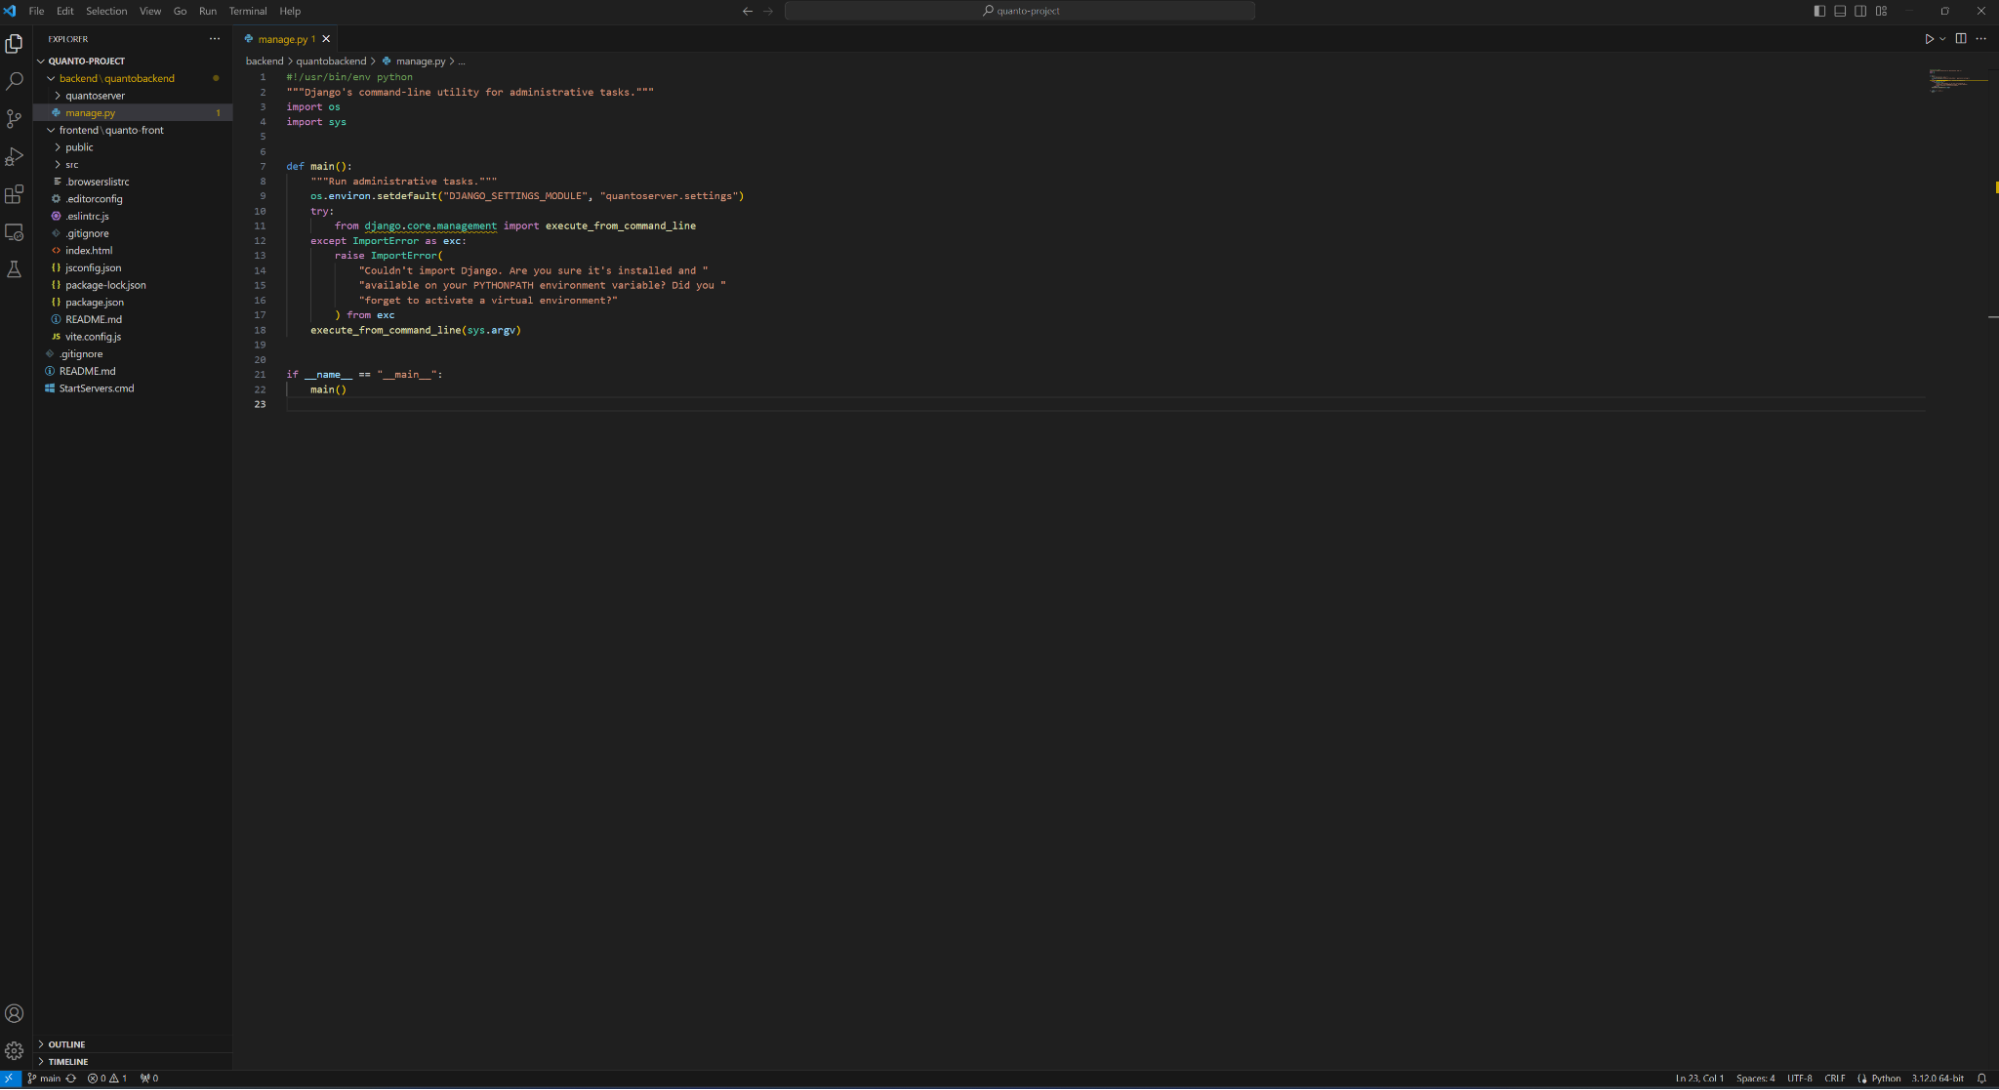
\includegraphics[width= \textwidth]{images/VS-Code.png}
        \caption{Screenshot VS-Code}
        \label{fig:beispiel}
    \end{figure}
    \subsection{Postman}
    Zum Testen der Backend API wird Postman genutzt. Postman ist sowohl als lokale Anwendung nutzbar, als auch als Webanwendung oder als Plug-in VS-Code. Postman ermöglicht es dazu noch das man seine Collections in einem Team zusammen bearbeiten und teilen kann

    \begin{figure}[h]
        \centering
        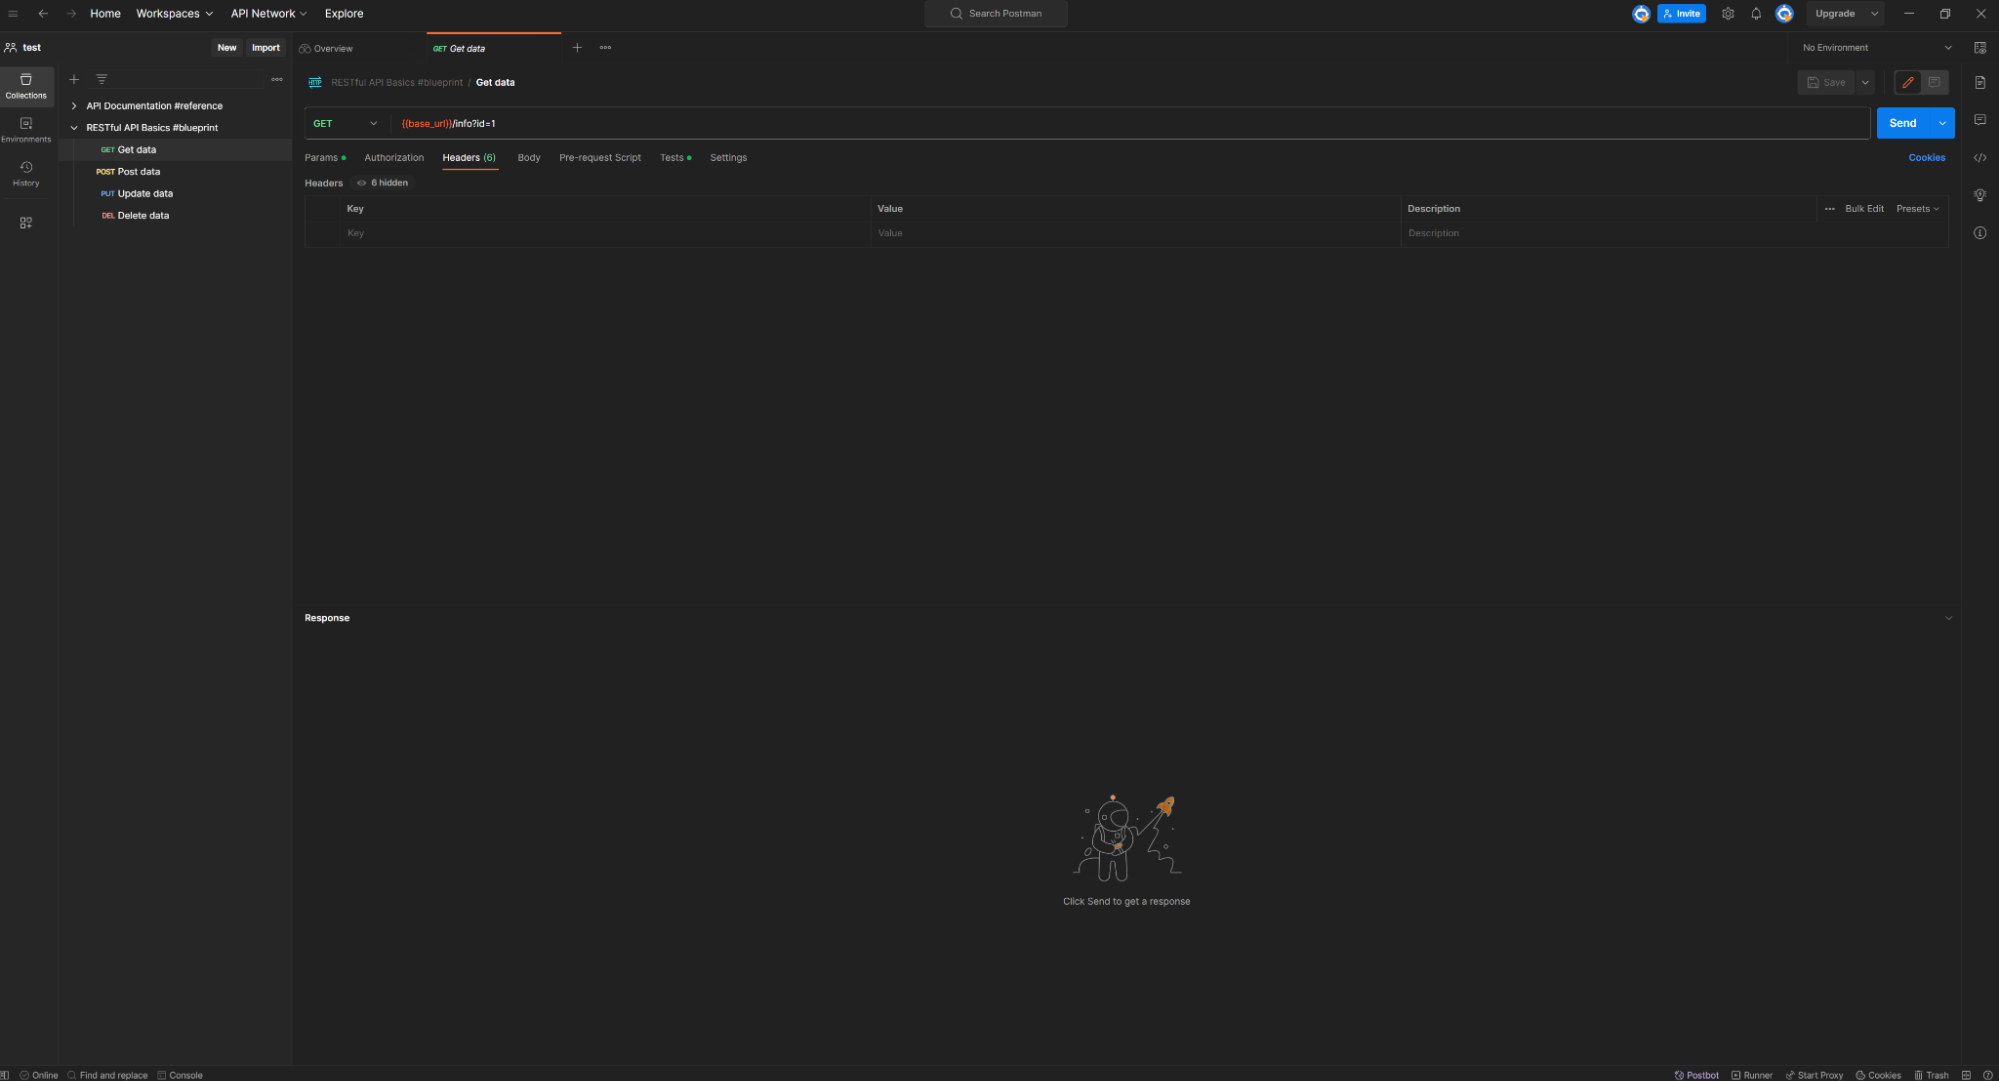
\includegraphics[width= \textwidth]{images/Postman.png}
        \caption{Screenshot Postman}
        \label{fig:beispiel}
    \end{figure}
    \subsection{Figma}
    Zum Erstellen unserer Mockups wird die Software Figma genutzt, da diese es ermöglicht, im Team gleichzeitig an Entwürfen zu arbeiten. Als erstes gab es die Entscheidung, welche Farbe für das Mockup genutzt werden sollte. Dabei hatten wir die Wahl zwischen einem orangen oder blauen Mockup, da diese sehr gut zum Stil von Quanto Solutions passen. Nach verschiedenen Tests haben wir uns entschieden, ein blaues Mockup zu erstellen. Die verschiedenen Screens werden im Folgenden gezeigt und näher erläutert. Der Login-Screen (Abbildung ), wo sich der Nutzer mit der Mitarbeiternummer und einem selbst gewählten Passwort einloggen kann, dient dazu, dass keine Person außerhalb der Firma Zugang erhält.

    \subsection{Microsoft SQL Server Managment Studio}
    Zum Verwalten, Interagieren und Entwickeln unserer Datenbank nutzen wir Microsoft SQL Server Management Studio, da dieses Programm von Microsoft selbst stammt und wir sowohl die Datenbank als auch die Verwaltungssoftware für diese aus einer Hand haben.

    \begin{figure}[h]
        \centering
        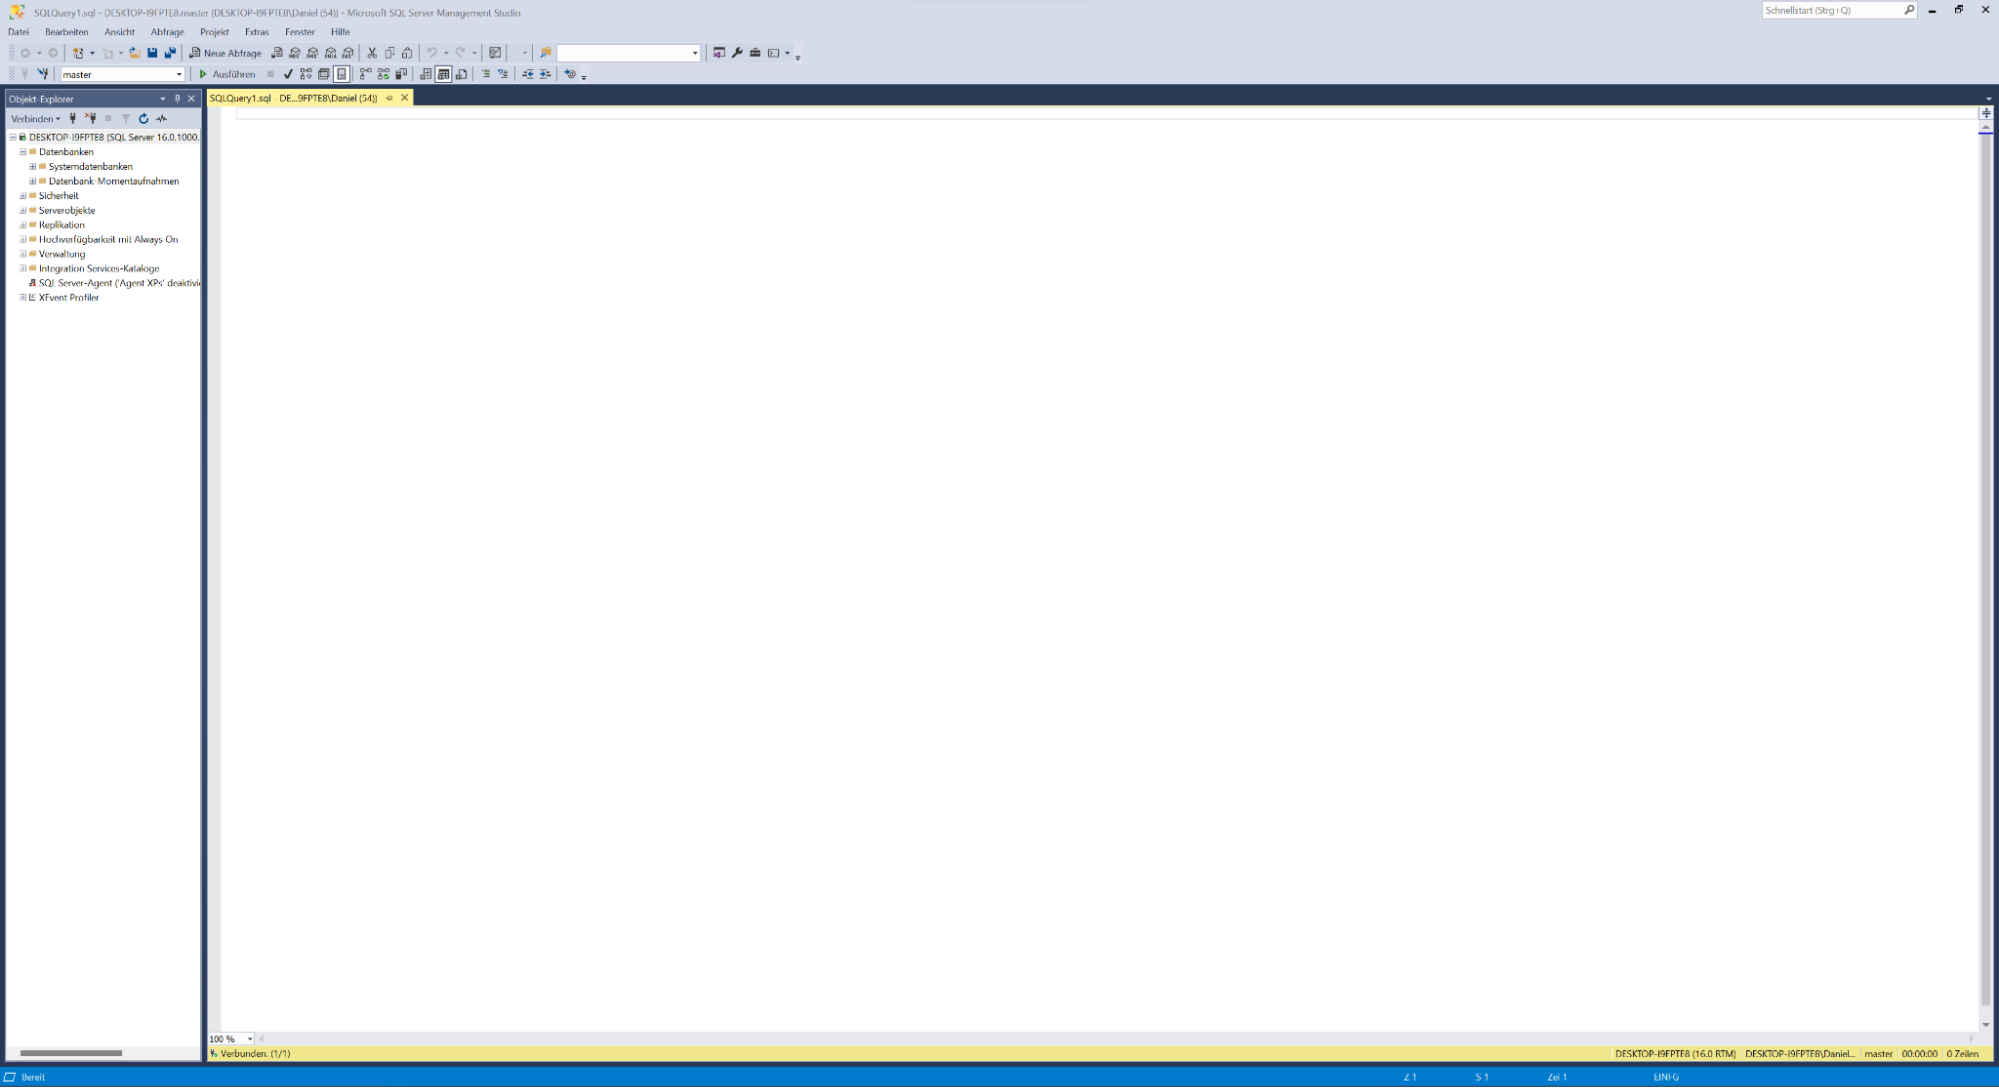
\includegraphics[width= \textwidth]{images/Microsoft SQL Server Management Studio.png}
        \caption{Screenshot Micorosoft SQL Server Managment Studio}
        \label{fig:beispiel}
    \end{figure}
    \subsection{Frontend: Vue.js}
    \subsection{Datenbank: Microsoft SQL Server}
    \subsection{Authentifizierung SAP}
    \subsection{Projektmanagment Jira}
    Warum wir Jira als Kommunikationstool nutzen:
    
    Wir setzen Jira als unser Kommunikationstool in unser Softwareprojekt ein, weil es sich als äußerst effizientes und vielseitiges Werkzeug für die interne und externe Kommunikation erwiesen hat. Wir nutzen Jira, um Informationen, Aufgaben, Fehler und Anforderungen in unseren Projekten zentral zu verwalten, was die Klarheit und Effizienz in der Projektarbeit fördert.
    \begin{enumerate}
        \item In Jira können wir in Echtzeit zusammenarbeiten und auf Aktualisierungen sowie Kommentare zugreifen, was eine schnelle und nahtlose Kommunikation unabhängig von den Standorten unserer Teammitglieder ermöglicht.
        \item Die Anpassungsfähigkeit von Jira erlaubt es uns, Arbeitsabläufe und Prozesse exakt auf unsere Projektanforderungen zuzuschneiden und benutzerdefinierte Felder hinzuzufügen, um projektbezogene Informationen effizient zu verfolgen.
        \item Die Verwendung von Jira steigert die Transparenz und Nachverfolgbarkeit in unseren Projekten, indem alle Teammitglieder einen klaren Überblick über den aktuellen Stand und den Fortschritt der Aufgaben haben.

    \end{enumerate}
    Vorteile unsere Vorgehensweise mit Jira
    \begin{enumerate}
        \item Jira ermöglicht eine effiziente Planung und Priorisierung von Aufgaben und Anforderungen, indem wir Arbeitsabläufe und Sprints definieren und den Fortschritt leicht im Blick behalten.
        \item Es erleichtert die detaillierte Meldung und Verfolgung von Softwarefehlern, was die Qualität unserer Software maßgeblich steigert.
        \item Wir können Aufgaben klar zuweisen und Verantwortlichkeiten definieren, um sicherzustellen, dass jedes Teammitglied weiß, welche Aufgaben es zu erfüllen hat.
        \item Jira fördert die Echtzeitkommunikation und den Austausch von Kommentaren zu Aufgaben und Anforderungen, was die Zusammenarbeit und den reibungslosen Informationsfluss im Team unterstützt.
        \item 
        Die umfassende Rückverfolgbarkeit von Anforderungen, Aufgaben und Problemen in Jira ist von großer Bedeutung in der Softwareentwicklung, um sicherzustellen, dass alle Anforderungen vollständig und termingerecht erfüllt werden.
    \end{enumerate}

\newpage
    

\section{Aufwandsschätzung}
    Da dieses Projekt im Rahmen des Moduls “Projekt Softwaretechnik und Medieninformatik” im Studiengang Softwaretechnik und Medieninformatik an der Hochschule Esslingen stattfindet, gibt es einen vorgeschriebenen Aufwand von 10 ECTS pro Person was 300 Stunden entspricht. Da das Team, welches dieses Projekt umsetzt, aus 5 Personen besteht, gibt es insgesamt 1500 Stunden, die in diesem Projekt verteilt werden können. Wir messen den Aufwand in Personentagen (PT), welche jeweils 8 Arbeitsstunden beinhalten. Dadurch kommen wir auf ein Gesamt Pensum von 187,5 PT, welches von der Hochschule vorgeschrieben ist.
    Bei der Methode der Aufwandsschätzung haben wir uns für die Bottom-Up-Methode entschieden. Hierbei arbeiten wir die Anforderungen des Projekts durch und schätzen für jede den entsprechenden Arbeitsaufwand.
    
    Die Aufwandsschätzung verteilt sich bei diesem Projekt dabei folgendermaßen:
    
    Um die einzelnen Anforderungen abzuarbeiten, brauchen wir erstmal ein Grundgerüst unserer Software, auf dem wir dann aufbauen können.

    \begin{enumerate}
        \item Frontend anlegen: 5PT
        \item Backend anlegen: 5PT
        \item Datenbank anlgegen: 5PT
        \item Prototyp eines Login-Systems implementieren und die Anforderung: “Die vorgesehenen Funktionalitäten für Manager PM und Mitarbeiter müssen jeweils nur für die jeweils nur für die jeweiligen Personen zur Verfügung stehen”: 5PT
    \end{enumerate}

    Im folgenden werden die Anforderungen geschätzt die auf dem Grundgerüst aufbauen

    \begin{enumerate}
        \item SAP Login einrichten: 15PT
        \item Manager müssen Projekte anlegen können (Kunde, Projektname, Budget, Zeitraum): 10PT
        \item Manager müssen für Projekte Projektmanager (PM) festlegen und Mitarbeiter zuordnen können: 15PT
        \item PM müssen auf Tagesebene eine zeitliche Einsatzplanung vornehmen und Mitarbeiter zuordnen können: 30PT
        \item Mitarbeiter müssen ihre IST-Aufwände buchen können. Zudem sollen Mitarbeiter dafür einen Reminder erhalten: 30PT
        \item Tagessätze Vor Ort und Remote unterscheiden sich! Jeweils eine Rechnungsposition: 5PT
        \item Arbeitspensum wird jeweils für Vor-Ort und Remote getrennt festgelegt: 5PT
        \item Es soll automatisiert eine Rechnung erzeugt werden und per E-Mail an die Rechnungsstellung geschickt werden: 10PT
        \item Puffer zm flexibel einteilen: 27,5 PT


    \end{enumerate}

\newpage

\section{Mockup}

        \begin{figure}[h]
            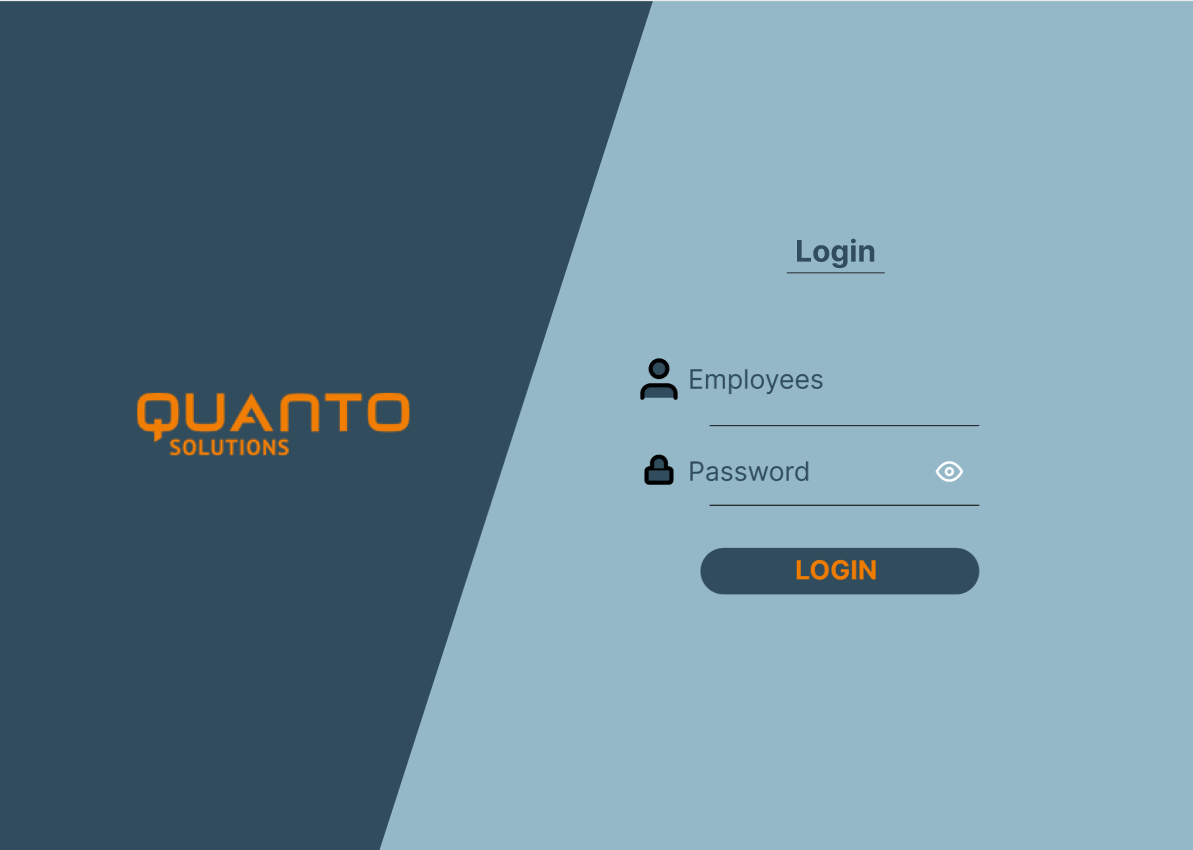
\includegraphics[height= 0.5\textwidth,width= \textwidth]{images/Login.png}
            \caption{Login-Ansicht}
            \label{fig:beispiel}
        \end{figure}
         \begin{figure}[h]
            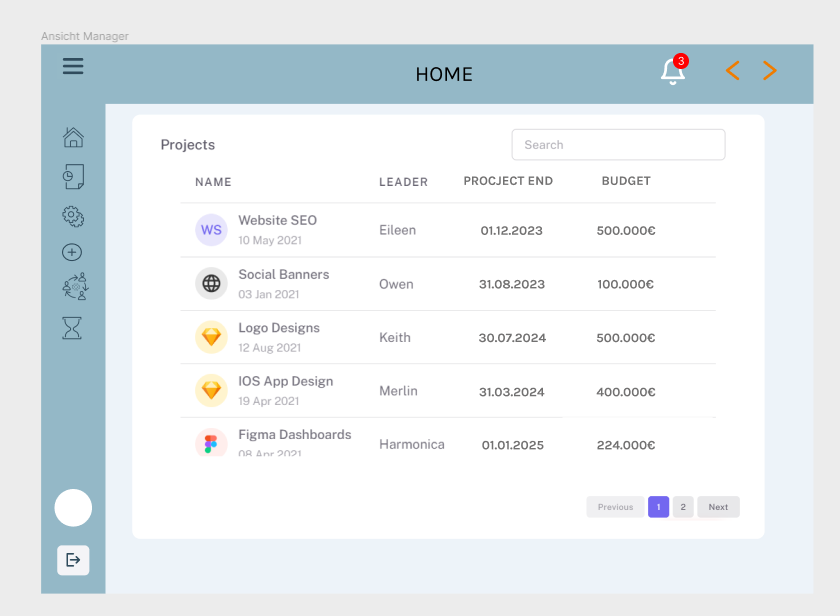
\includegraphics[height= 0.5\textwidth,width= \textwidth]{images/Home.png}
            \caption{Home-Ansicht}
            \label{fig:beispiel}
        \end{figure}
        

\newpage
         \begin{figure}[h]
            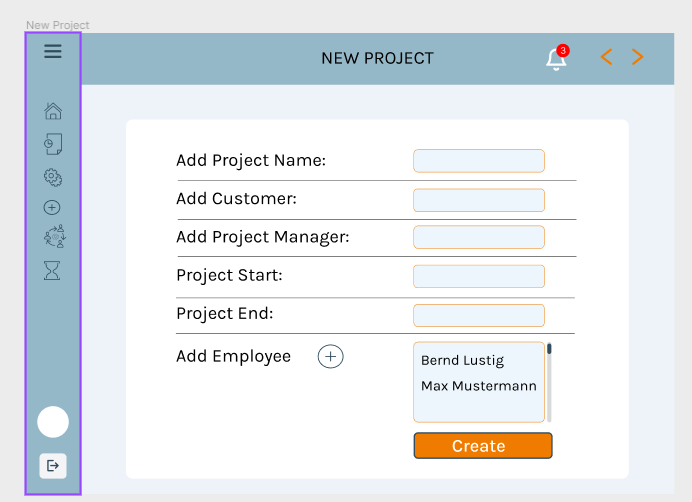
\includegraphics[height= 0.5\textwidth,width= \textwidth]{images/New Project.png}
            \caption{New Project Ansicht}
            \label{fig:beispiel}
        \end{figure}

         \begin{figure}[h]
            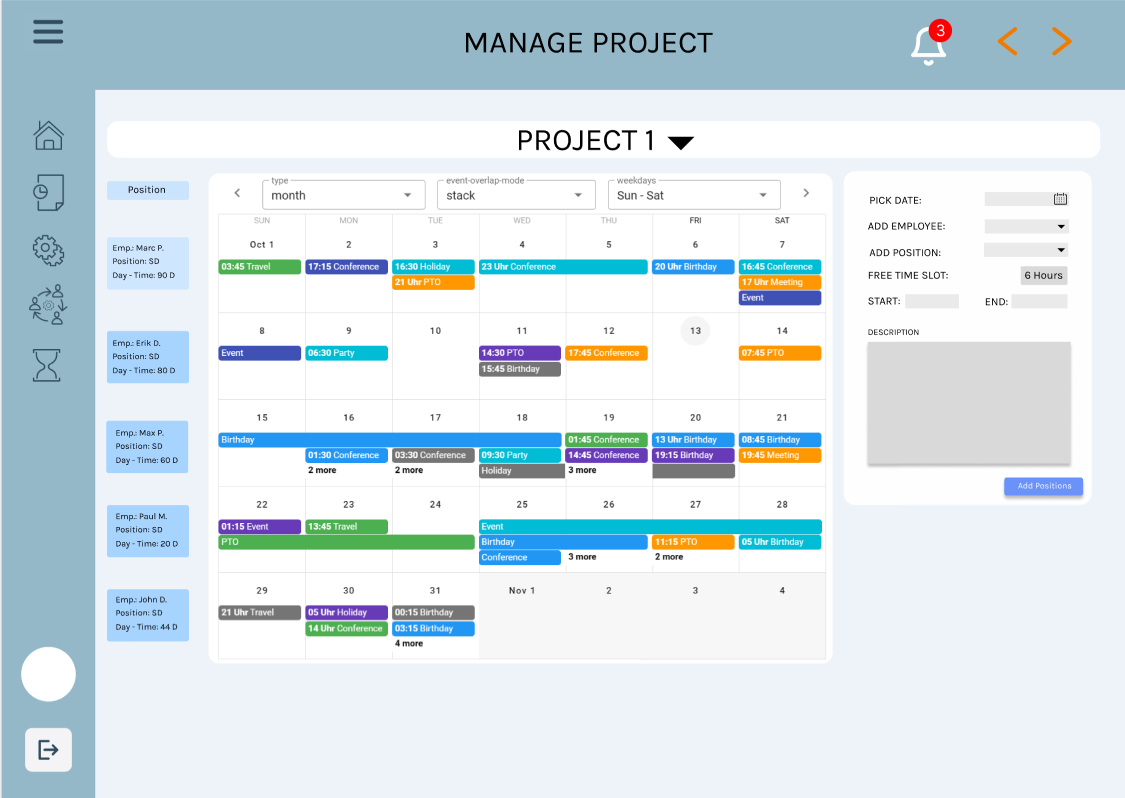
\includegraphics[height= 0.5\textwidth,width= \textwidth]{images/Manage Project.png}
            \caption{Manage-Project-Ansicht}
            \label{fig:beispiel}
        \end{figure}
        
\newpage
         \begin{figure}[h]
            \includegraphics[height= 0.5\textwidth,width= \textwidth]{images/Positionen einfügen.png}
            \caption{Position-Einfügen Ansicht}
            \label{fig:beispiel}
        \end{figure}

         \begin{figure}[h]
            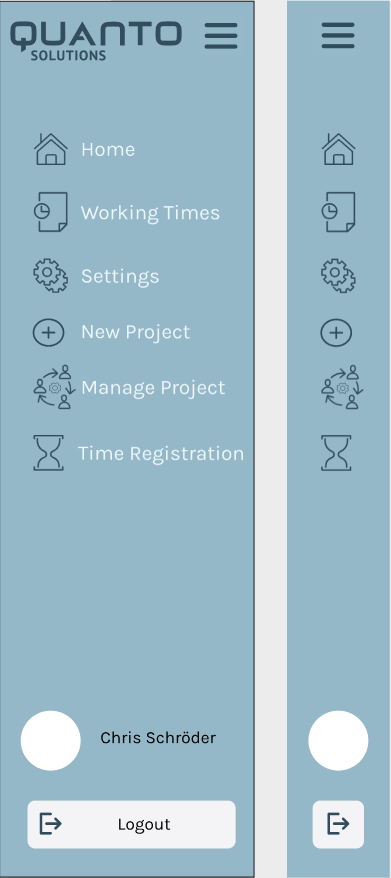
\includegraphics[height= 0.5\textwidth,width= \textwidth]{images/Sidebar.png}
            \caption{Sidebar-Ansicht}
            \label{fig:beispiel}
        \end{figure}

\newpage
         \begin{figure}[h]
            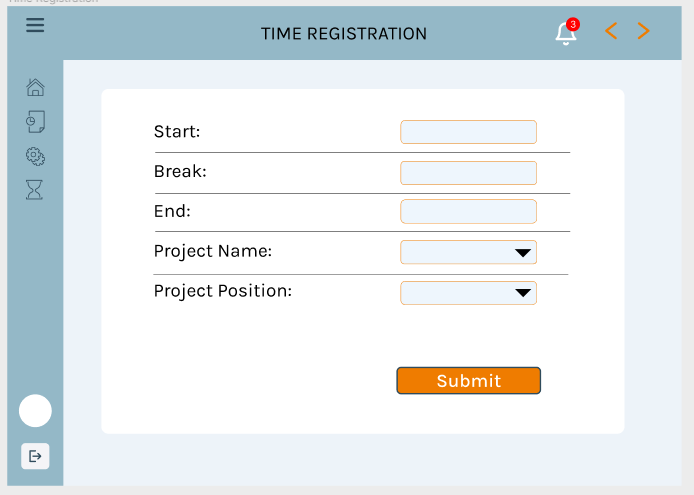
\includegraphics[height= 0.5\textwidth,width= \textwidth]{images/Time Registration.png}
            \caption{Time Registration Ansicht}
            \label{fig:beispiel}
        \end{figure}

        \begin{figure}[h]
            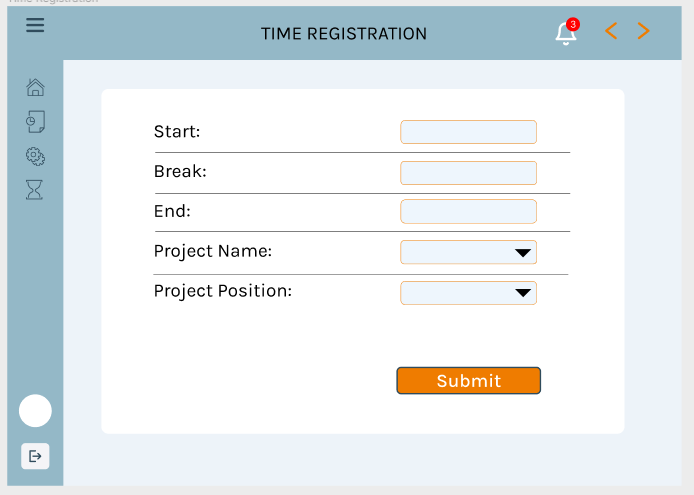
\includegraphics[height= 0.5\textwidth,width= \textwidth]{images/Time Registration.png}
            \caption{Working Times Ansicht}
            \label{fig:beispiel}
        \end{figure}
\newpage

\section{Datenbank}

    \begin{figure}[h]
        \centering
        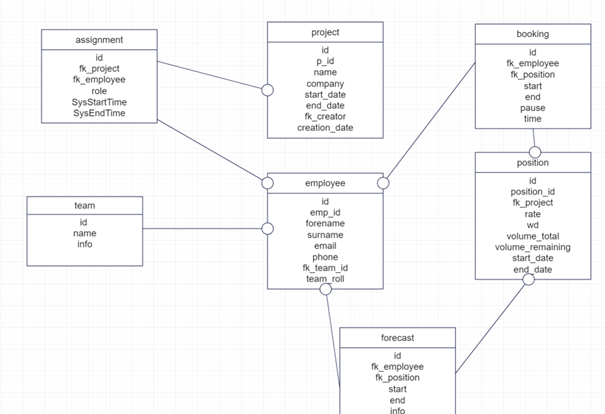
\includegraphics[width= \textwidth]{images/logischeAnsicht.png}
        \caption{Logische Sicht Datenbank}
        \label{fig:beispiel}
    \end{figure}

    \begin{figure}[h]
        \centering
        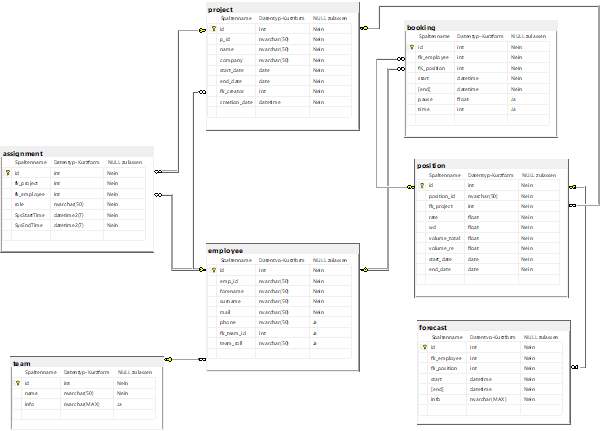
\includegraphics[width= \textwidth]{images/datenbankphysisches-Layout.png}
        \caption{Physisches Layout Datenbank}
        \label{fig:beispiel}
    \end{figure}

\newpage

    \subsection{Tabellen}

        \subsubsection{Employee}
        \begin{lstlisting}[language=Sql, caption= Create Table Statement für Employee Table]
    CREATE TABLE [dbo].[employee] (
    [id]         INT           IDENTITY (1, 1) NOT NULL,
    [emp_id]     NVARCHAR (50) NOT NULL,
    [forename]   NVARCHAR (50) NOT NULL,
    [surname]    NVARCHAR (50) NOT NULL,
    [mail]       NVARCHAR (50) NOT NULL,
    [phone]      NVARCHAR (50) NULL,
    [fk_team_id] INT           NULL,
    [team_roll]  NVARCHAR (50) NULL,
    CONSTRAINT [PK_employee] PRIMARY KEY CLUSTERED ([id] ASC),
    CONSTRAINT [FK_employee_team] FOREIGN KEY ([fk_team_id]) REFERENCES 
    [dbo].[team] ([id])
);
        \end{lstlisting}
        \subsubsection{Team}
         \begin{lstlisting}[language=Sql, caption= Create Table Statement für Team Table]
    CREATE TABLE [dbo].[team] (
    [id]   INT            IDENTITY (1, 1) NOT NULL,
    [name] NVARCHAR (50)  NOT NULL,
    [info] NVARCHAR (MAX) NULL,
    CONSTRAINT [PK_team] PRIMARY KEY CLUSTERED ([id] ASC)
);

         \end{lstlisting}
        \subsubsection{Project}
        \begin{lstlisting}[language=Sql, caption= Create Table Statement für Project Table]
    CREATE TABLE [dbo].[project] (
    [id]            INT           IDENTITY (1, 1) NOT NULL,
    [p_id]          NVARCHAR (50) NOT NULL,
    [name]          NVARCHAR (50) NOT NULL,
    [company]       NVARCHAR (50) NOT NULL,
    [start_date]    DATE          NOT NULL,
    [end_date]      DATE          NOT NULL,
    [fk_creator]    INT           NOT NULL,
    [creation_date] DATETIME      NOT NULL,
    CONSTRAINT [PK_project] PRIMARY KEY CLUSTERED ([id] ASC),
    CONSTRAINT [FK_project_creator] FOREIGN KEY ([fk_creator]) 
    REFERENCES [dbo].[employee] ([id])
);
         \end{lstlisting}
        \subsubsection{Position}
        \begin{lstlisting}[language=Sql, caption= Create Table Statement für Position Table]
    CREATE TABLE [dbo].[position] (
    [id]               INT           IDENTITY (1, 1) NOT NULL,
    [position_id]      NVARCHAR (50) NOT NULL,
    [fk_project]       INT           NOT NULL,
    [rate]             FLOAT (53)    NOT NULL,
    [wd]               FLOAT (53)    NOT NULL,
    [volume_total]     FLOAT (53)    NOT NULL,
    [volume_remaining] FLOAT (53)    NOT NULL,
    [start_date]       DATE          NOT NULL,
    [end_date]         DATE          NOT NULL,
    CONSTRAINT [PK_position] PRIMARY KEY CLUSTERED ([id] ASC),
    CONSTRAINT [FK_position_project] FOREIGN KEY ([fk_project]) 
    REFERENCES [dbo].[project] ([id])
);
         \end{lstlisting}
        \subsubsection{Assignment}
        \begin{lstlisting}[language=Sql, caption= Create Table Statement für Assignment Table]
    CREATE TABLE [dbo].[assignment] (
    [id]          INT           IDENTITY (1, 1) NOT NULL,
    [fk_project]  INT           NOT NULL,
    [fk_employee] INT           NOT NULL,
    [role]        NVARCHAR (50) NOT NULL,
    CONSTRAINT [PK_assignment] PRIMARY KEY CLUSTERED ([id] ASC),
    CONSTRAINT [FK_assignment_employee] FOREIGN KEY ([fk_employee]) REFERENCES
    [dbo].[employee] ([id]),
    CONSTRAINT [FK_assignment_project] FOREIGN KEY ([fk_project]) REFERENCES
    [dbo].[project] ([id])
    );
    GO
    CREATE UNIQUE NONCLUSTERED INDEX [Index_Assignment_Id]
    ON [dbo].[assignment]([id] ASC);


         \end{lstlisting}
        \subsubsection{Booking}
        \begin{lstlisting}[language=Sql, caption= Create Table Statement für Booking Table]
    CREATE TABLE [dbo].[booking] (
    [id]          INT        IDENTITY (1, 1) NOT NULL,
    [fk_employee] INT        NOT NULL,
    [fK_position] INT        NOT NULL,
    [start]       DATETIME   NOT NULL,
    [end]         DATETIME   NOT NULL,
    [pause]       FLOAT (53) NULL,
    [time]        INT        NULL,
    CONSTRAINT [PK_tracking] PRIMARY KEY CLUSTERED ([id] ASC),
    CONSTRAINT [FK_tracking_employee] FOREIGN KEY ([fk_employee]) REFERENCES
    [dbo].[employee] ([id]),
    CONSTRAINT [FK_tracking_position] FOREIGN KEY ([fK_position]) REFERENCES
    [dbo].[position] ([id])
);


         \end{lstlisting}
        \subsubsection{Forecast}
        \begin{lstlisting}[language=Sql, caption= Create Table Statement für Forecast Table]
    CREATE TABLE [dbo].[forecast] (
    [id]          INT            IDENTITY (1, 1) NOT NULL,
    [fk_employee] INT            NOT NULL,
    [fk_position] INT            NOT NULL,
    [start]       DATETIME       NOT NULL,
    [end]         DATETIME       NOT NULL,
    [info]        NVARCHAR (MAX) NOT NULL,
    CONSTRAINT [PK_plan] PRIMARY KEY CLUSTERED ([id] ASC),
    CONSTRAINT [FK_plan_position] FOREIGN KEY ([fk_position]) REFERENCES 
    [dbo].[position] ([id])
);


         \end{lstlisting}

    Der SQL Code zum erstellen der Datenbank inklusive der Tabellen, ist im Github-Repository des Backends zu finden.

\newpage

\section{Schnittstellen Definition}

    \subsection{Datenbank Backend}
    Für die Schnittstelle zwischen der Datenbank und dem Backend haben wir uns für die Micosoft ODBC Schnittstelle entschieden. Diese kann wiefolgt beschrieben werden.
    
    "Die Microsoft Open Database Connectivity (ODBC)-Schnittstelle ist eine C-Programmiersprachenschnittstelle, mit der Anwendungen über eine Vielzahl von Datenbankverwaltungssystemen (DBMSs) auf Daten zugreifen können. ODBC ist eine schnittstelle mit niedriger Leistung, die speziell für relationale Datenspeicher entwickelt wurde."\cite{MSODBC}.

    \begin{figure}[h]
        \centering
        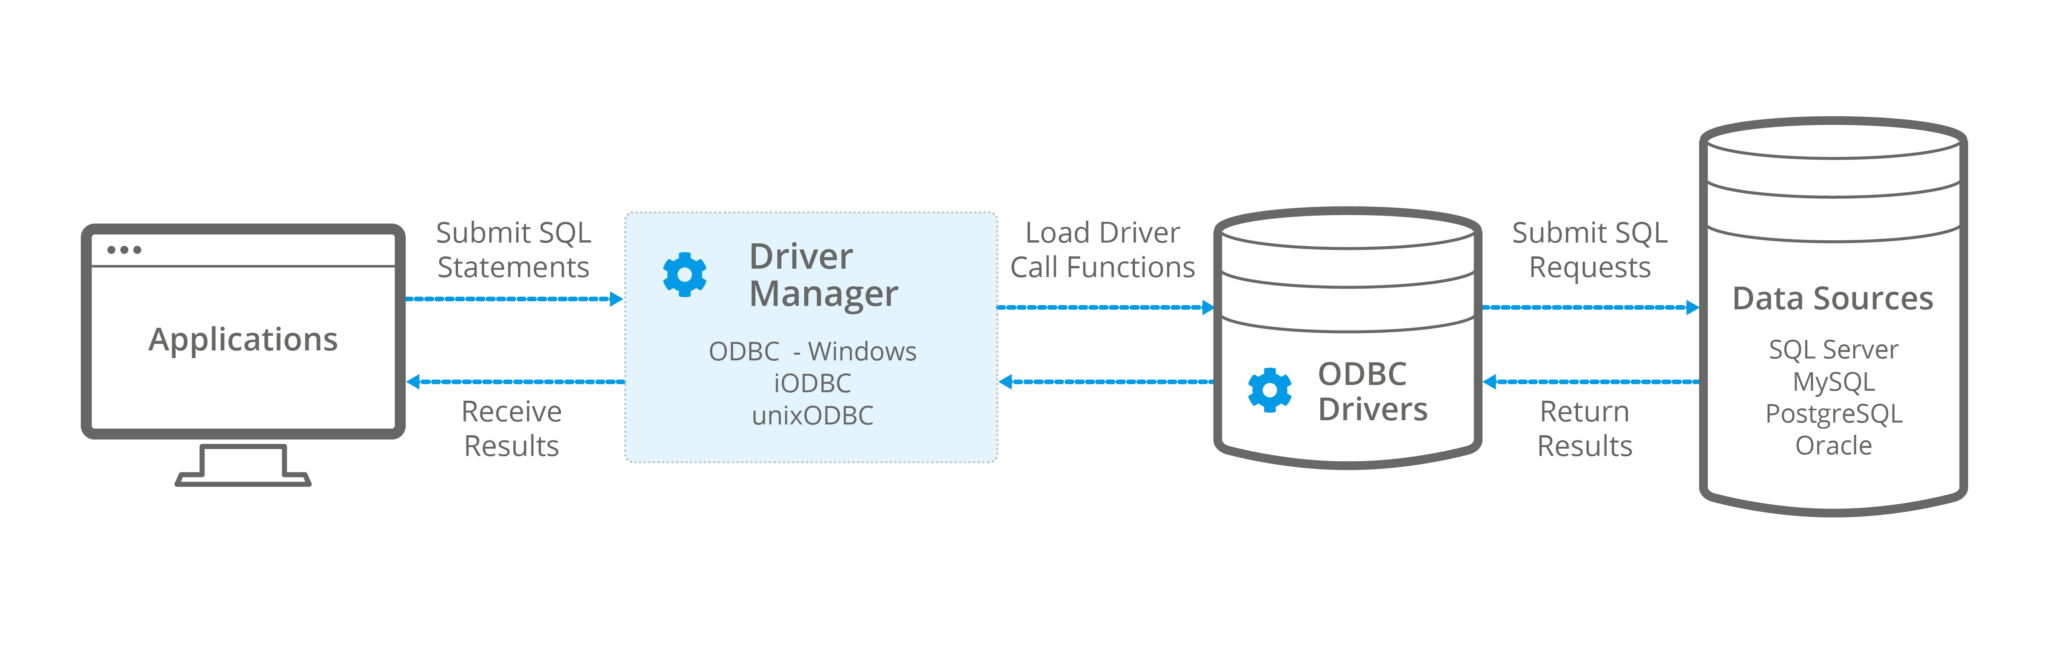
\includegraphics[width= \textwidth]{images/odbc.png}
        \caption{Veranschaulichung ODBC Schnittstelle}
        \label{fig:beispiel}
        \cite{ODBC}
    \end{figure}

    Die ODBC Schnittstelle bietet dabei für uns mehrere Vorteile. Auch wenn in diesem Projekt als Datenbank Microsoft SQL Server verwendet wird, besteht die Möglichkeit das auch eine andere Datenbank-Technologie verwendet wird, solange diese ebenfalls die ODBC Schnittstelle unterstützt. Dadurch vergrößert sich die potenzielle Zielgruppe unseres Projekts, da für den Fall dass potenzielle Nutzer andere Datenbank-Systeme präferieren und verwenden wollen. Ein weiterer Vorteil der sich ergibt ist die Plattformunabhängigkeit, wodurch das Projekt auf allen gängigen Betriebssystemen laufen kann.
    

    
    \subsection{Backend Frontend}
    Als Schnittstelle zwischen dem Backend und Frontend wird eine REST-Api verwendet. Dies ist die Konsequenz aus der Entscheidung für das Backend Framework, da es sich dabei um ein Framework handelt, welches eine REST-API implementiert, und wir daran nichts ändern, da die REST-API viele Vorteile für uns bietet.

    \begin{figure}[h]
        \centering
        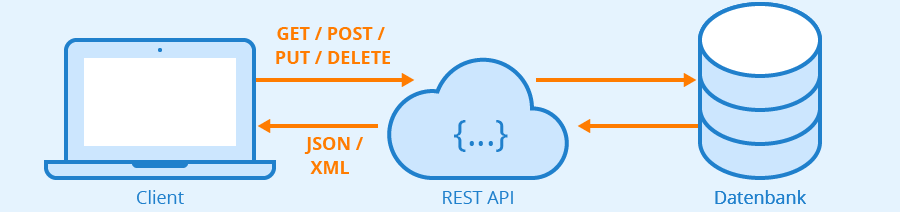
\includegraphics[width= \textwidth]{images/Rest-API.png}
        \caption{Veranschaulichung REST-API}
        \label{fig:beispiel}
        \cite{REST}
    \end{figure}
    

\newpage

\section{Protokoll}
    \subsection{1. Woche, Zeitraum 02.10.2023-08.10.2023}
    Im Meeting am  06.10.2023 wurden folgenden Sachen hinsichtlich des Projektes festgelegt: 
    
    Quanto Solutions gab uns keine Vorgaben in Hinsicht auf Technologien und Programmiersprachen, mit der Einschränkung, dass es sich dabei um eine Webanwendung handeln muss, was sich jedoch auch aus den Vorgaben des SWTM-Moduls ergab. Somit wurde uns freie Hand gelassen im Aspekt auf die technischen Entscheidungen. Zudem wurde noch einmal genau auf die Anforderungen des Projektmanagement Tools eingegangen. Diese wurden unterteilt in Muss-, Soll- und Kann-Anforderungen. Des Weiteren wurde besprochen, wie ein Projekt aufgebaut ist und welche verschiedenen Rollen in diesem involviert sind. Dadurch wurde noch einmal deutlich gemacht, dass jede Rolle in einem Projekt verschiedene Zugriffsrechte hat.  Bis zum nächsten Meeting sollten wir ein Mockup erstellen.

    \subsection{2. Woche Zeitraum 09.10.2023 -22.10.2023}
    Im Meeting am 13.10 wurden folgende Sachen hinsichtlich des Projektes festgelegt.
    
    Zur Zeiterfassung der Mitarbeiterzeiten wird die Start- und Endzeit des Arbeitstages inklusive Pausenzeiten, manuell von Hand eingetragen und nicht, wie im ersten Mockup, per Start- und Stop-Button gestoppt. Für das Eintragen der Arbeitszeiten wurde vereinbart, dass Mitarbeiter ihre Arbeitszeiten auf Stundenbasis eintragen können und nicht, wie bisher gedacht, nur ganze Tage buchen können. In Hinsicht auf das nachträgliche Ändern von Arbeitszeiten wurde festgelegt, dass die Arbeitszeiten bis zum Ende des Monats geändert werden können.
    Des Weiteren wurde festgehalten, dass Manager in Projekten alle Berechtigungen besitzen. Die Projektsprache hinsichtlich der User Interfaces wurde auf Englisch festgelegt, damit möglichst viele Mitarbeiter diese verwenden können, hinsichtlich der möglichen Akquisition von internationalen Firmen. Ebenfalls wurde festgelegt, dass die App-Sidebar auf jeder Seite der App sichtbar sein soll, um eine möglichst effektive und schnelle Navigation in der App zu gewährleisten.
    Hinsichtlich der Planung von Projekten in der Anwendung wurde festgehalten, dass Manager die Positionen erstellen. Der Projektleiter kann dann Mitarbeiter für diese Positionen zuordnen und auf Tagesbasis das Projekt planen.

    \subsection{3.Woche Zeitraum 16.10.2023 - 22.1.2023}
    Im Meeting am 20.10 wurden folgende Sachen hinsichtlich des Projektes festgelegt.
    
    Es wurde vom Kunden das blaue Farbschema für das Produkt gewünscht. Zudem wurde sich auch gewünscht, wenn möglich, die Positionen in “Add Employee” per Drag and Drop zu veranschaulichen. Doch da haben wir die endgültige Entscheidung, weswegen wir und auch für das Drag and Drop Feature entschieden haben. Bei “Manage Project” sollen alle Mitarbeiter angezeigt werden und diese eine begrenzung von 8 Stunden pro Tag haben. Dabei soll man diese Mitarbeiter direkt für mehrere Tage, Wochen und Monate einplanen können. Das soll man wiederholen, zum Beispiel per Checkbox und im Kalender auch rauslöschen können. Eine Tagessicht wurde ebenfalls vereinbart. 
    In “Time Registration” haben wir beschlossen das Mitarbeiter am Ende des Monats ihre Zeiten bestätigen können und diese dann der Projektleiter sehen kann. Die Mitarbeiter können somit frei im Monat ihre Stunden anpassen. Nach dem bestätigen der Zeiten kann der Mitarbeiter eine Zeiten nicht mehr ändern, weswegen bei vergessen der Eintragung, die Zeiten händisch durch den Projektleiter erfolgen müssen.

    \subsection{4. Woche Zeitraum: 23.10.203 -29.10.2023}
    Im Meeting am 27.10 wurden folgende Sachen hinsichtlich des Projektes festgelegt.
    
    In Bezug auf unser Kanban-Board wurde festgelegt die User Stories in kleinere Tasks zu zerlegen. Es wurde zudem festgelegt das wir 2 GitHub Repositories haben sollen, wobei die erste für das Frontend ist und die zweite für das Backend.
    Zur Code Dokumentation wurde gesagt das wir ein einheitlichen Kommentierstil haben sollen.
    In Bezug auf das Datenbankmodell sollten ein paar Änderungen vorgenommen werden, wie die Team Employee Tabelle zu entfernen und eine TeamId anzulegen. Diese sollten angepasst werden. Es kam die Frage auf für den SQL Server einen Docker zu verwenden, welches bis zum nächsten Meeting von der Kundenseite beantwortet werden soll.
    Der Kalender in “Manage Project” ist zu viel des Guten und könnte auch durch eine einfache Tabelle dargestellt werden. Laut dem Kunden ist es unsere Entscheidung zu sagen ob wir ein Kalender oder eine Tabelle erstellen. Dabei spielt beim einplanen die Uhrzeit keine Rolle, sondern nur die 8 Stunden. Es wurde vereinbart bis nächste Woche Dienstag ein MockUp in Form einer Tabelle zu erstellen.

    \subsection{5. Woche Zeitraum: 30.10.2023 - 05.11.2023}
        Im Meeting am 31.10 wurden folgende Sachen hinsichtlich des Projektes festgelegt.
    Zwischen dem Kalender und der Tabelle haben wir uns entschieden eine Tabelle zu machen und diese mit Vuetify Komponenten und Usability Features wie Drag and Drop zu erstellen. Dabei soll die Benutzerfreundlichkeit auf Stundenbasis auch verbessert werden. Hinzu kommt, dass wir bis Freitag, den 03.11, den Mockup abschließen sollen.
    Es wurde endgültig entschieden, beim Einplanen der Mitarbeiter per Tabelle, diese für bis zu 8 Stunden einplanen zu können. Als Zusatzfeature mit geringerer Priorität können wir eine Wiederholung der Planung erstellen, wo die Planung dann z.B. für jeden Montag der nächsten 2 Monate gilt.
    Beim Datenmodell wurden einige Tabellen geändert und es wurde festgelegt das Datenmodell bis zum nächsten Meeting als Bild bereitzustellen, damit der Kunde sich dazu Gedanken machen kann. 
    Des Weiteren wurde festgehalten, Docker Container für jeweils das Frontend, Backend sowie für die Datenbank zu erstellen.
    Es wurde festgelegt einen zentralen Ort für die Protokolle zu haben und diese nach dem jedem Meeting mit dem Kunden zu teilen.
    
    Im Meeting am 3.11 wurden folgenden Sachen hinsichtlich des Projektes festgelegt.
    Datenbank:
    Bei der Nutzung und Erstellung der Datenbank sollten keine Kosten entstehen, sie sollte lizenzfrei sein. Das Projekt ist ein Open-Source-Projekt.
    Dokumentation Datenbank: Die SQL Statements sollen ins Git hinzugefügt werden (Backend) Repository. In der Doku soll das Datenbankmodell hinzugefügt und erklärt werden.
    Datenbankmodell:
    Das Datenbankmodell muss noch einmal überarbeitet werden. In der Projekttabelle soll folgendes hinzugefügt werden: Projekt Ersteller, Datum wann das Projekt erstellt wurde, und wer der Projektmanager ist. In der Tabelle Employees soll das Attribut: team roll auf title umbenannt werden. Außerdem soll mit passenden Präfixen gearbeitet werden, zum Beispiel fk  bei Foreign Keys. Um die Bezeichnung eindeutig zu machen, müssen noch alle Attribute, die auf Deutsch sind, auf Englisch umbeannt werden.
    
    
    
    
    Mockup:
    Zusammen sind wir noch einmal das Mockup durchgegangen und haben letzte Anpassungen vorgenommen:
    Es wurde beschlossen, dass nichts dagegen spricht, dass der Projektleiter auch das Budget sehen kann für seine Projekte.
    Dem Manager soll bei der Projekterstellung auch das kalkulierte Budget angezeigt werden, bevor er das Projekt anlegt.
    Die Manage Project Ansicht: Soll eine Tabelle sein in der alle Mitarbeiter aufgelistet sind die diesem Projekt zugeteilt wurden: Folgendes soll in der Tabelle angezeigt werden: Eine Spalte mit bereits eingeplante Stunden über alle Projekte des Mitarbeiters dadurch kann man sehen wie viele Stunden man der Mitarbeiter an dem Tag noch einplanen könnte. In der nächsten Spalte kann man dann die Anzahl der Stunden eintragen, wie viele Stunden man den Mitarbeiter an diesem Tag einplanen möchte. Sowie eine Spalte Positionen, in dem man festlegt, auf welcher Position der Mitarbeiter an diesem Tag eingeplant werden soll.
    Diese Liste soll immer einen kompletten Monat umfassen und man kann per DropDown Menü bequem zwischen den Monaten hin und her wechseln.
    Die Working Times Ansicht: Soll auch nun auch in einer Tabelle dargestellt werden wie die Manage Project Ansicht, für ein besseres Look and Feel und eine bessere Übersichtlichkeit.
    Zudem soll es eine neue Extra-Ansicht geben, in dem der Mitarbeiter seine Zeiten sieht, die er noch nicht erfasst hat, obwohl er an diesen Tagen eingeplant war. Hier hat er noch die Möglichkeit, seine Zeiten manuell nachzutragen. Zudem kann der Mitarbeiter seine Zeiten am Monatsende bestätigen, nachdem er alles kontrolliert hat. Sobald er Sie bestätigt hat, kann er keine Änderungen mehr vornehmen. Sobald seine Arbeitszeiten bestätigt wurden, landen diese beim Projekt Manager, nur er kann jetzt noch Änderungen vornehmen.
    Bis zum nächsten Meeting sollten wir mit der Implementierung starten und schauen, dass wir das Frontend mit dem Backend und der Datenbank verbinden. Um erste Einträge in der Software vorzunehmen.
    (Nice to have: Mange Project Ansicht: Mitarbeiter anklicken um Extra Infos zu erhalten, in welchen anderen Projekten der Mitarbeiter noch involviert ist.)

    \subsection{6. Woche Zeitraum 06.11.2023-12.11.2023}
        Teambesprechung mit Andre: Protokoll vom 10.11.2023, 14:00 Uhr bis 15:00 Uhr
        
    Die heutige Teambesprechung mit Andre fokussierte sich auf entscheidende Aspekte der Authentifizierung, Softwarearchitektur und Meilensteinplanung. Besonderes Augenmerk wurde auf die SAP-Integration gelegt, wobei unterschiedliche Berechtigungen je nach Rolle diskutiert wurden. Im Bereich der Softwarearchitektur standen die Planung von Meilensteinen sowie die Schnittstellenbeschreibung mittels OpenAPI SWAGGER im Vordergrund. Ein weiterer Schwerpunkt lag auf der technischen Durchführung und Containerisierung, einschließlich der Ankündigung von Meilensteinen und dem Backend-Zugriff auf Datenbanken.
    Des Weiteren wurde die Vorbereitung für Meilenstein 2 thematisiert, einschließlich der Inhalte und Terminvereinbarungen. Die Besprechung lieferte einen klaren Fahrplan für die Umsetzung der vereinbarten Maßnahmen bis zum nächsten Meeting.
    Teambesprechung mit Lisa: Protokoll vom 10.11.2023, 15:00 Uhr bis 16:00 Uhr
    
    Im Anschluss an die Besprechung mit Andre stand die Teambesprechung mit Lisa im Fokus. Das Team setzte sich intensiv mit der Gestaltung einer neuen Tabelle in Figma auseinander. Dabei wurden das Modell und die Ansicht der Tabelle überprüft und diskutiert. Besondere Aufmerksamkeit galt der Filterung nach Personen, der Gestaltung der Positionsspalte und der Farbgebung basierend auf der Stundenanzahl. Die Diskussion über die unabhängige Funktionalität und die spätere Verbindung rundete die Besprechung ab.
    Diese Zusammenfassung bietet einen klaren Überblick über die behandelten Themen und dient als Grundlage für die Umsetzung der festgelegten Maßnahmen bis zum nächsten Meeting.



\newpage

\bibliographystyle{IEEEtran}
\bibliography{quellen}



\end{document}
